% !TEX root = btstack_gettingstarted.tex
\section{Protocols and Profiles}
\label{section:protocols_profiles}

BTstack implements following Bluetooh protocols: HCI, L2CAP, L2CAP-LE, RFCOMM, SDP, SMP,  and ATT, as well as three profiles: GATT, GAP and SPP, see Figure \ref{fig:BTstackProtocolArchitecture}. 

\begin{figure}[htbp] %  figure placement: here, top, bottom, or page
   \centering
   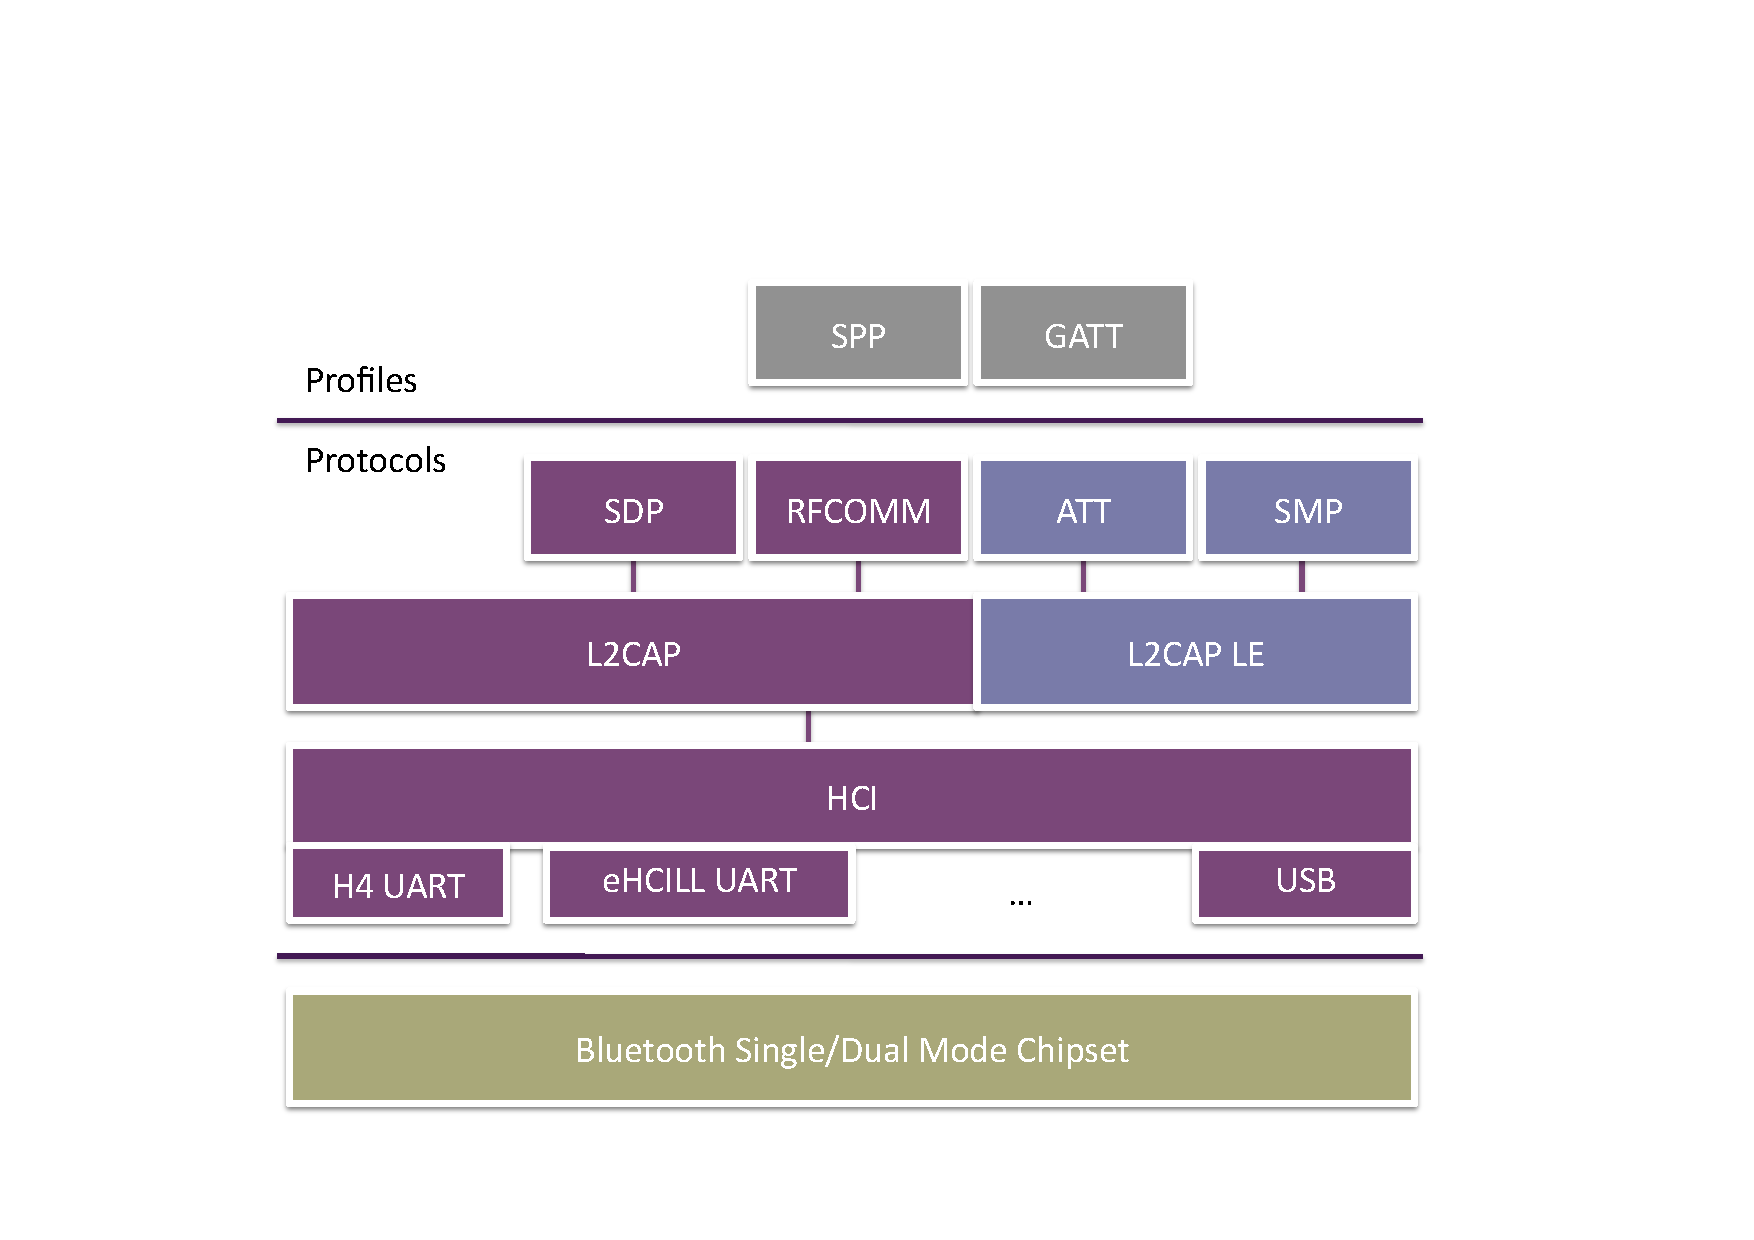
\includegraphics[width=0.7\textwidth]{picts/btstack-protocols.pdf} 
   \caption{BTstack Protocol Architecture}
   \label{fig:BTstackProtocolArchitecture}
\end{figure}

\subsection{HCI - Host Controller Interface}
The HCI protocol provides a command interface to the Bluetooth chipset. 

\subsection{L2CAP -  Logical Link Control and Adaptation Protocol}
The L2CAP protocol supports higher level protocol multiplexing and packet fragmentation.
%\section{Security Levels and L2AP}

\subsection{L2CAP LE - L2CAP Low Energy Protocol}
The L2CAP LE variant is optimized for connectionless data used by Bluetooth Low Energy devices. It is the base for the Attribute Protocol (ATT) of Bluetooth LE, which defines how to discover, read, and write attributes on a peer device. % , and the conveying of quality of service information. - L2CAP _can_ do this, but BTstack does not

\subsection{RFCOMM - Radio Frequency Communication Protocol}
The Radio frequency communication (RFCOMM) protocol provides emulation of serial ports over the L2CAP protocol.
and reassembly. 
\subsubsection{RFCOMM flow control}
\label{section:flowcontrol}
RFCOMM has a mandatory credit-based flow-control. This means that two devices that established RFCOMM connection, use credits to keep track of how many more RFCOMM data packets can be sent to each. If a device has no (outgoing) credits left, it cannot send another RFCOMM packet, the transmission must be paused. During the connection establishment, initial credits are provided. BTstack tracks the number of credits in both directions. If no outgoing credits are available, the RFCOMM send function will return an error, and you can try later. For incoming data, BTstack provides channels and services with and without automatic credit management via different functions to create/register them respectively. If the management of credits is automatic, the new credits are provided when needed relying on ACL flow control - this is only useful if there is not much data transmitted and/or only one physical connection is used. If the management of credits is manual, credits are provided by the application such that it can manage its receive buffers explicitly. 
\subsubsection{RFCOMM configuration - TODO}
\todo{rfcomm configuration}
%\subsection{add RFCOMM port configuration for both local and remote}
%\subsection{add RFCOMM modem and line status control/information}
%\subsection{add RFCOMM\_AGGREGATE\_FLOW\_OFF to recoverable RFCOMM send errors (example in tex, code)}
%\section{Security Levels and RFCOMM}

\subsection{SDP - Service Discovery Protocol}
The SDP protocol allows to discover services provided by a Bluetooth device. 

\subsection{SMP - Security Manager Protocol }
The SMP protocol allows to setup authenticated and encrypted connection.

\subsection{ATT - Attribute Protocol}
ATT is a wire application protocol, while GATT dictates how ATT is employed in service composition. Every Low Energy profile must be based on GATT. So, ultimately, every LE service uses ATT as the application protocol. An ATT server stores attributes. An ATT client stores nothing; it uses the ATT wire protocol to read and write values on server attributes. Most of the ATT protocol is pure client-server: client takes the initiative, server answers. But ATT has notification and indication capabilities, in which the server takes the initiative of notifying a client that an attribute value has changed, saving the client from having to poll the attribute.

\subsection{SPP - Serial Port Profile}
The SPP profile defines how to set up virtual serial ports and connect two Bluetooth enabled devices. See Appendix \ref{appendix:api_} for the SPP API.

\subsection{GAP - Generic Access Profile for Low Energy}
The GAP profile defines how to discover and how to connect to a Bluetooth device. There are several GAP roles that a Bluetooth device can take, but the most important ones are the Central and the Peripheral role. Peripheral devices are those that provide information or can be controlled and central devices are those that consume information or control the peripherals. Before the connection can be established, devices are first going through the advertising process. What happens with the peripheral device after the central device connect to a it, depends on the peripheral's Bluetooth controller. The peripheral will either stop advertising itself and other devices will no longer be able to see it or connect to it until the existing connection is broken, or it will be able to continue with advertising so that the parallel connections can be established.
\subsubsection{GAP BLE Roles}
There are four GAP roles defined for a Bluetooth low energy device: Broadcaster, Observer, Peripheral and Central. A device may operate in multiple GAP roles concurrently.
\begin{itemize}
\item \emph{GAP Broadcaster Role} - A broadcast device only sends advertisements and cannot be connected. It can emit some useful data as part of the advertisement. The most prominent use for this is Apple's iBeacon technology which uses broadcast devices to emit a unique ID. Apple's iOS framework then help to map this ID onto a specific location, e.g., in a museum. Broadcasting is efficient as no connection and no ATT database are needed. To control energy consumption the broadcast interval can be configured. An advertisement can contain up to 31 bytes of information. In addition, another 31 bytes of information can be sent in the scan response.
\item \emph{GAP Observer Role} - An observer device only receives advertising events and cannot be connected. 
\item \emph{GAP Central Role} - The role of the central device is to scan for peripherals, connect to them, and discover and receive data from them or sends data to control them. During scanning the central device can retrieve information on other device such are its name and unique number, as well as some broadcast data from its services. Upon connection, the central explores the device by discovering its primary and included services, characteristics, and characteristic descriptors.
\item \emph{GAP Peripheral Role} - The role of a peripheral device is to deliver information on their inputs, i.e. sensor values, battery level, current time, to the applications running on central devices. It can also receive a write request from a central device and control connected actors, e.g. turn on and set the color of the light. Peripherals can broadcast data, they can be discovered and connected to by a central device, they can stay also disconnected and then establish connection when needed. 
\end{itemize} 
\subsubsection{Advertising and Scan Response Data}
There are two ways to send advertising out with GAP: The Advertising Data payload and the Scan Response payload. Both payloads are identical and can contain up to 31 bytes of data, but only the advertising data payload is mandatory. The scan response payload is an optional secondary payload that central devices can request.
\subsubsection{Dedicated bonding}


\subsection{GATT - Generic Attribute Profile}
The GATT profile uses the ATT for discovering services, and for reading and writing characteristic values on a peer device. GATT also specifies the format of data contained on the GATT server: it groups ATT attributes into Services and Characteristics, and defines set of queries the GATT Client can use to discover services, characteristics.

\subsubsection{GATT BLE Roles}

\begin{itemize}
\item \emph{GATT Server Role} - The GATT server stores the data and accepts GATT client requests, commands and confirmations. The GATT server sends responses to requests and when configured, sends indication and notifications asynchronously to the GATT client. 
\item \emph{GATT Client Role} - The GATT Client is used to discover services, and their characteristics and descriptors on a peer device. It can also subscribe for notifications or indications that the characteristic on the GATT server has changed its value. 
\end{itemize}

\subsubsection{Attribute Database - GATT-based Profile Hierarchy}
Attributes, as transported by the Attribute Protocol, are formatted as services and characteristics. Services may contain a collection of characteristics. Characteristics contain a single value and any number of descriptors describing the characteristic value. The peripheral device server (ATT server) provides a set of attributes that are stored in a simple lookup database. GATT formats these attributes as services and characteristics. Services may contain a collection of characteristics. Characteristics contain a single value and any number of descriptors describing the characteristic value. A service starts with a service declaration attribute defining its type, i.e. primary or secondary. It is followed by the included services and characteristics. By means of including services, the service can incorporate more complex behavior, and still keep the definition small. A characteristic is assigned to a single value that can be accessed. It is composed of three basic elements: declaration, value and descriptors. The characteristic declaration defines how the data can be accessed. A characteristic descriptor is used to capture the additional properties, e.g., to configure if the characteristic value should be reported upon its change. Together, characteristic declaration and the descriptors define types of action that can be performed on characteristic value.

The security that is required to access a service or a characteristic is defined in ATT database along with service/characteristic declaration. The GATT Server usually does not initiate any security request, but it can. 

\subsection{BNEP -  Bluetooth Network Encapsulation Protocol}
The BNEP protocol is built on top of L2CAP and it is used to transport control and data packets over standard network protocols such as TCP, IPv4 or IPv6.  . BNEP specifies a minimum L2CAP MTU of 1691. 

\subsection{PAN -  Personal Area Networking Profile}
The PAN profile uses BNEP to provide on-demand networking capabilities between Bluetooth devices. The PAN profile defines the following roles:
\begin{itemize}
\item PAN User (PANU)
\item Network Access Point (NAP)
\item Group Ad-hoc Network (GN)
\end{itemize}

PANU is a Bluetooth device that communicates as a client with GN, or NAP, or with another PANU Bluetooth device, through a point-to-point connection. Either the PANU or the other Bluetooth device may terminate the connection at anytime.

NAP is a Bluetooth device that provides the service of routing network packets between PANU by using BNEP and the IP routing mechanism. A NAP can also act as a bridge between Bluetooth networks and other network technologies by using the Ethernet packets.

The GN role enables two or more PANUs to interact with each other through a wireless network without using additional networking hardware. The devices are connected in a piconet where the GN acts as a master and communicates either point-to-point or a point-to-multipoint with a maximum of seven PANU slaves by using BNEP.

Currently, BTstack supports only PANU.

\section{Dual Mode Support}
\subsection{BR/EDR - Basic Rate/Extended Data Rate, or shortly Classic}
\subsection{LE - Low Energy}
Bluetooth Low Energy (BLE) is a Bluetooth technology used for discovering services and optimized for low power consumption - you don't get high data rates, and usually don't keep connection for long periods. The focus is on two different device roles:  devices that provide services and/or can be controlled and devices that consume services and/or control other devices. Devices are first going through the advertising process that is governed by the Generic Access Profile (GAP). Once the connection is established, the communication will be governed by the Generic Attribute Profile (GATT). Both profiles, GAP and GATT, have concepts that describe these two BLE roles:  GAP defines Peripheral and Central, and GATT defines Server and Client role respectively. The GATT roles are not necessarily tied to specific GAP roles and may be specified by higher layer profiles. GATT is built on top of the Attribute Protocol (ATT), which defines how to discover, read, and write attributes on a peer device. In addition, BLE uses two more BT protocols: SMP for for pairing and transport specific key distribution and L2CAP LE variant optimized for connectionless data used by Bluetooth Low Energy devices. 


\subsubsection{Private/random addresses}
To better protect privacy, a LE device can choose use a private i.e. random Bluetooth address. This address changes at a user-specified rate. To allow for later reconnection, the central and peripheral devices exchange their Identity Resolving Keys (IRKs) during bonding. The IRK is used to verify if a new address belongs to a previously bonded device.

\subsubsection{Security manager}
\label{section:security_manager}